\documentclass[../../dd.tex]{subfiles}
% Document
\begin{document}
    \chapter{User Interface Design}


    \section{Overview}
    In this section are present some screenshots of \textit{Baddy} mobile application.
    During the design and development, the attention was focused on the mobile
    application, even if the application is developed to adapt itself to different screen sizes.


    \section{Screens}
    \begin{figure}[H]
        \centering
        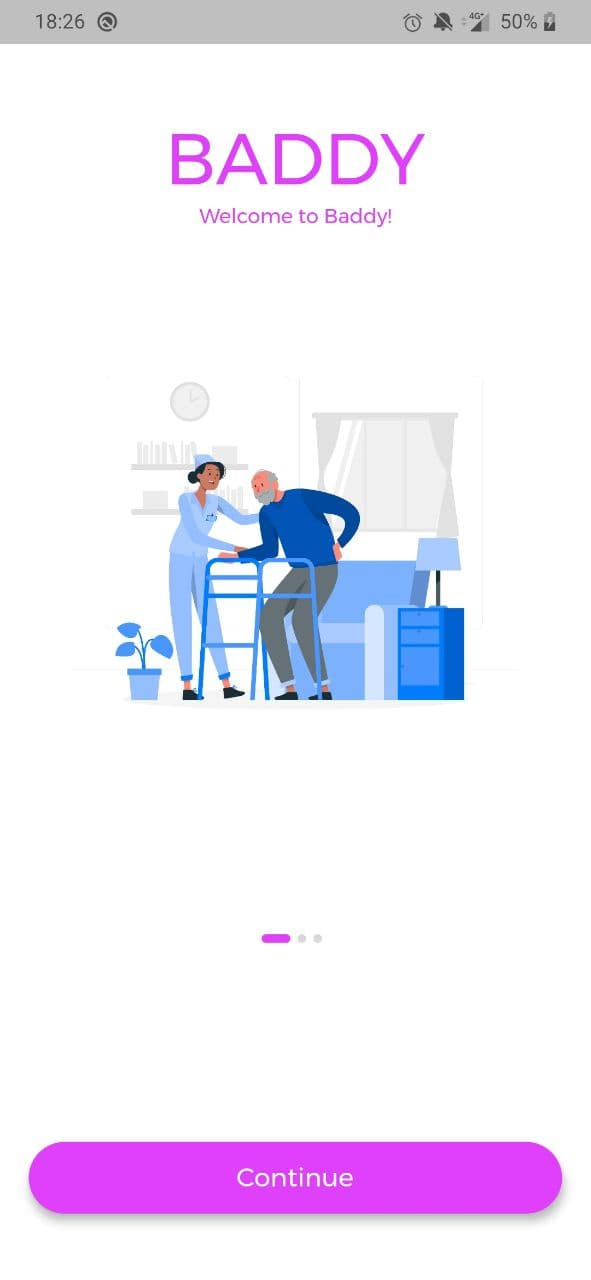
\includegraphics[height=.4\textheight]{../../assets/screens/splash1.jpg}
        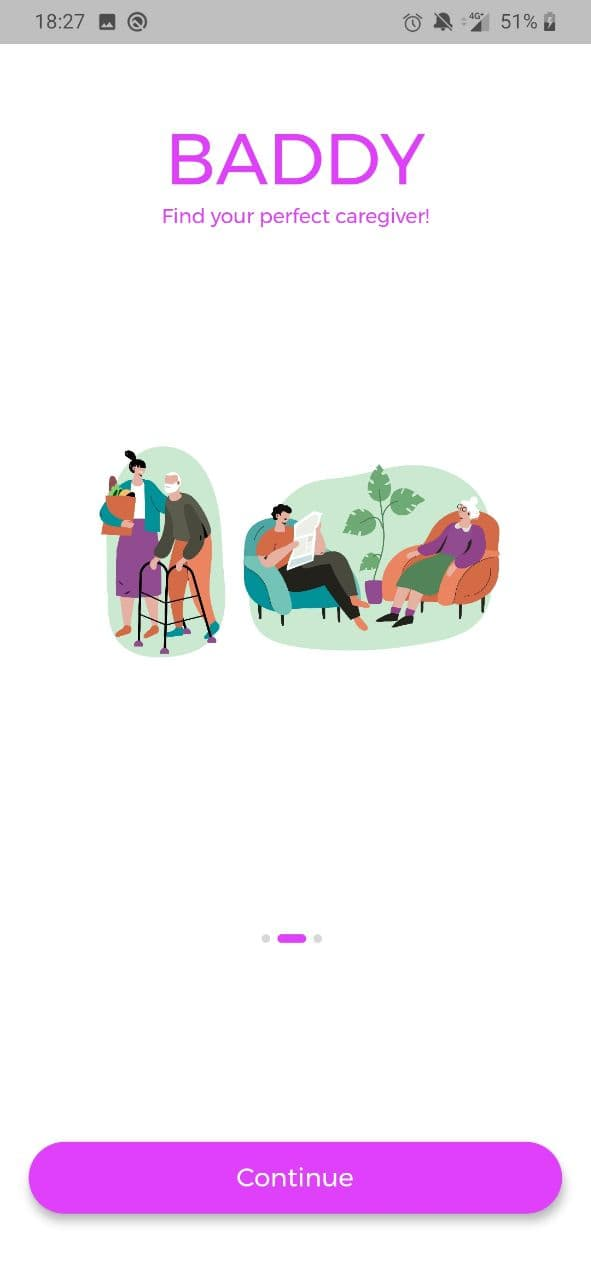
\includegraphics[height=.4\textheight]{../../assets/screens/splash2.jpg}
        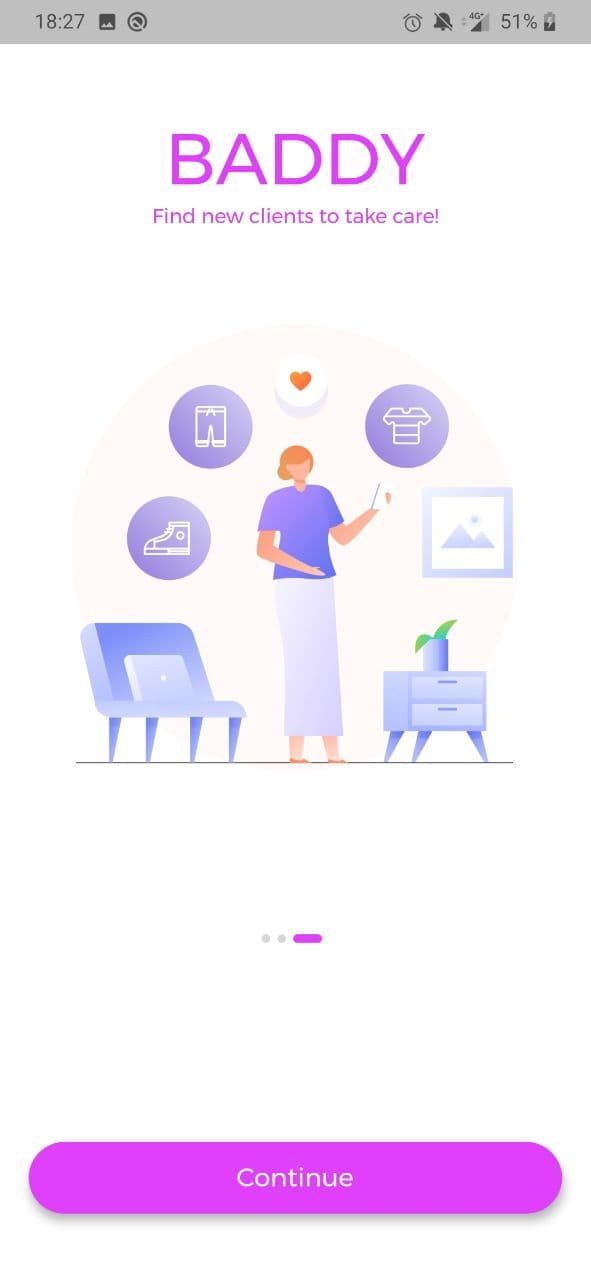
\includegraphics[height=.4\textheight]{../../assets/screens/splash3.jpg}
        \caption{\textbf{Splash Screen}}\label{fig:figure}
    \end{figure}
    \begin{center}
        The \textbf{Splash Screen} is the first screen that will show up if you open the app for the first time.
    \end{center}

    \begin{figure}[H]
        \centering
        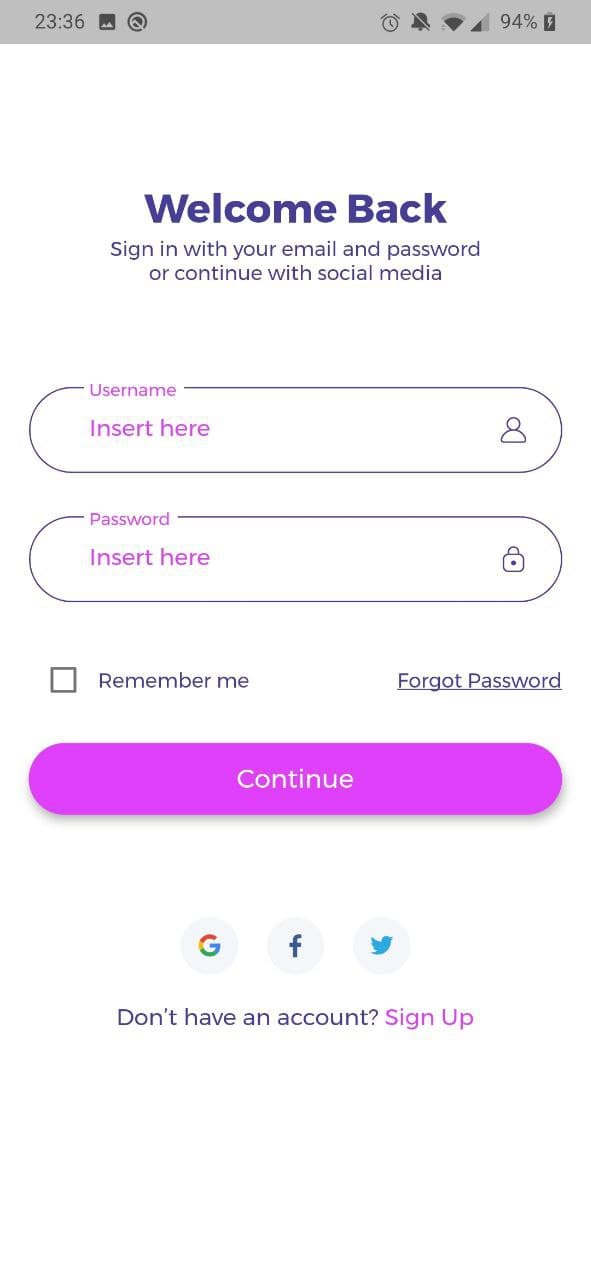
\includegraphics[height=.6\textheight]{../../assets/screens/login.jpg}
        \caption{\textbf{Login Screen}}\label{fig:figure}
    \end{figure}
    \begin{center}
        The \textbf{Login Screen} is the first screen that will show up when the application is loaded if not already logged in.
    \end{center}

    \begin{figure}[H]
        \centering
        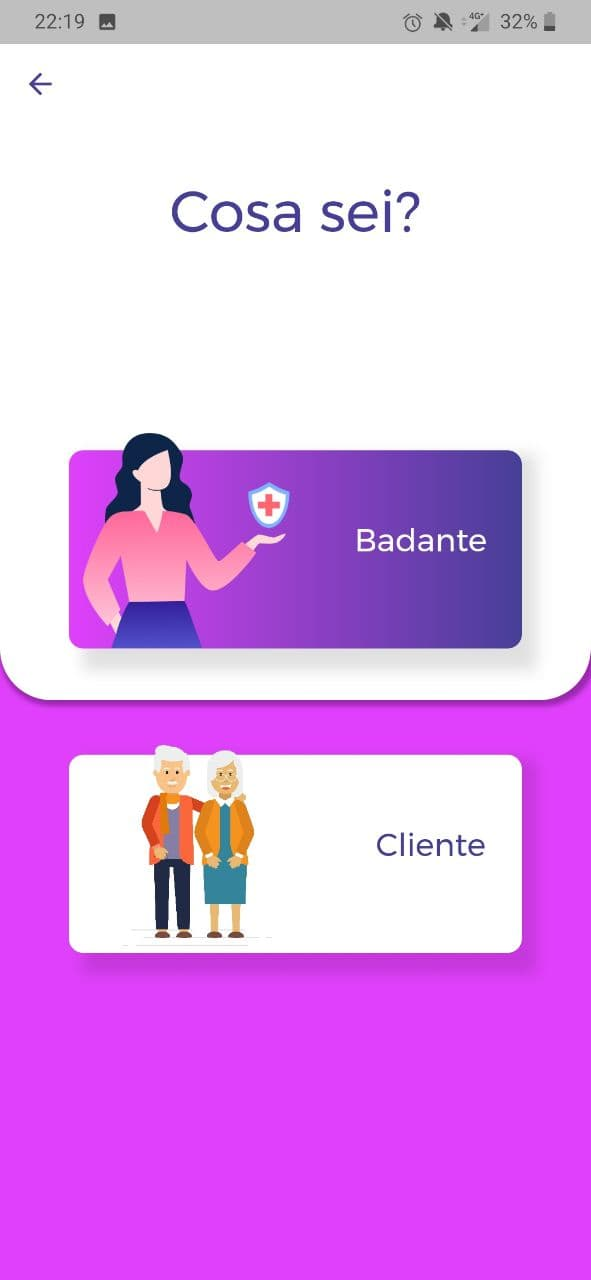
\includegraphics[height=.6\textheight]{../../assets/screens/role.jpg}
        \caption{\textbf{Choose Role Screen}}\label{fig:figure}
    \end{figure}
    \begin{center}
        The \textbf{Choose Role Screen} shows up as soon as the user taps on `sign up` in the \textit{Login Screen}.
        Here the user must choose between standard user and caregiver.
    \end{center}

    \begin{figure}[H]
        \centering
        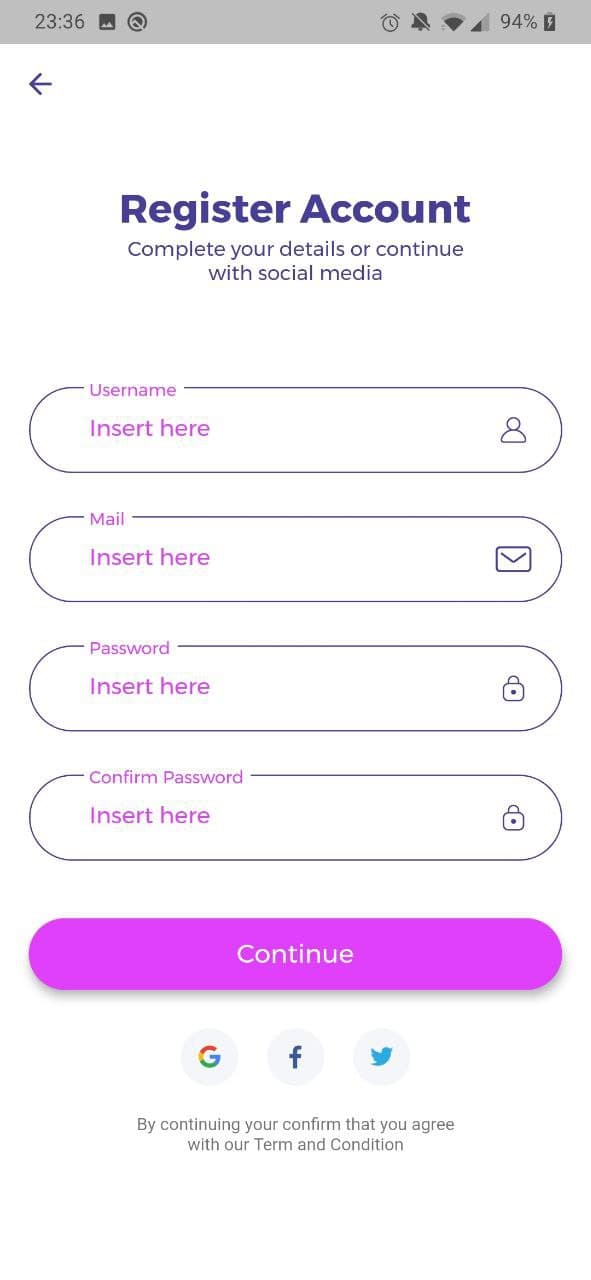
\includegraphics[height=.6\textheight]{../../assets/screens/register.jpg}
        \caption{\textbf{Sign Up Screen}}\label{fig:figure}
    \end{figure}
    \begin{center}
        The \textbf{Sign Up Screen} appears after choosing the role.
        Here the user must insert mandatory data in order to proceed.
        This step is the same for both standard user and caregivers.
    \end{center}

    \begin{figure}[H]
        \centering
        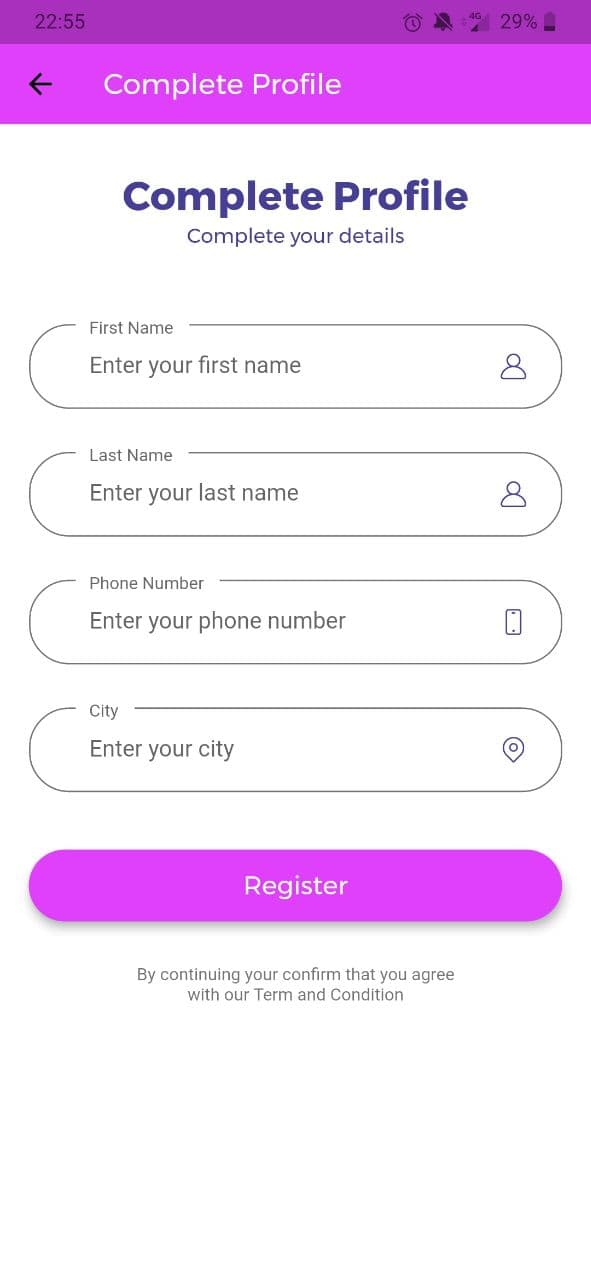
\includegraphics[height=.6\textheight]{../../assets/screens/complete.jpg}
        \caption{\textbf{Complete Registration Screen}}\label{fig:figure}
    \end{figure}
    \begin{center}
        The \textbf{Complete Registration Screen} shows up only if the chosen role is the caregiver.
        Here more mandatory info are required in order to complete the registration.
    \end{center}

    \begin{figure}[H]
        \centering
        
\includegraphics[height=.6\textheight]{../../assets/screens/success.jpg}
        \caption{\textbf{Success Screen}}\label{fig:figure}
    \end{figure}
    \begin{center}
        The \textbf{Success Screen} appears if all the steps for the registration are done correctly.
        From here you can easily access the homepage by clicking the button.
    \end{center}

    \begin{figure}[H]
        \centering
        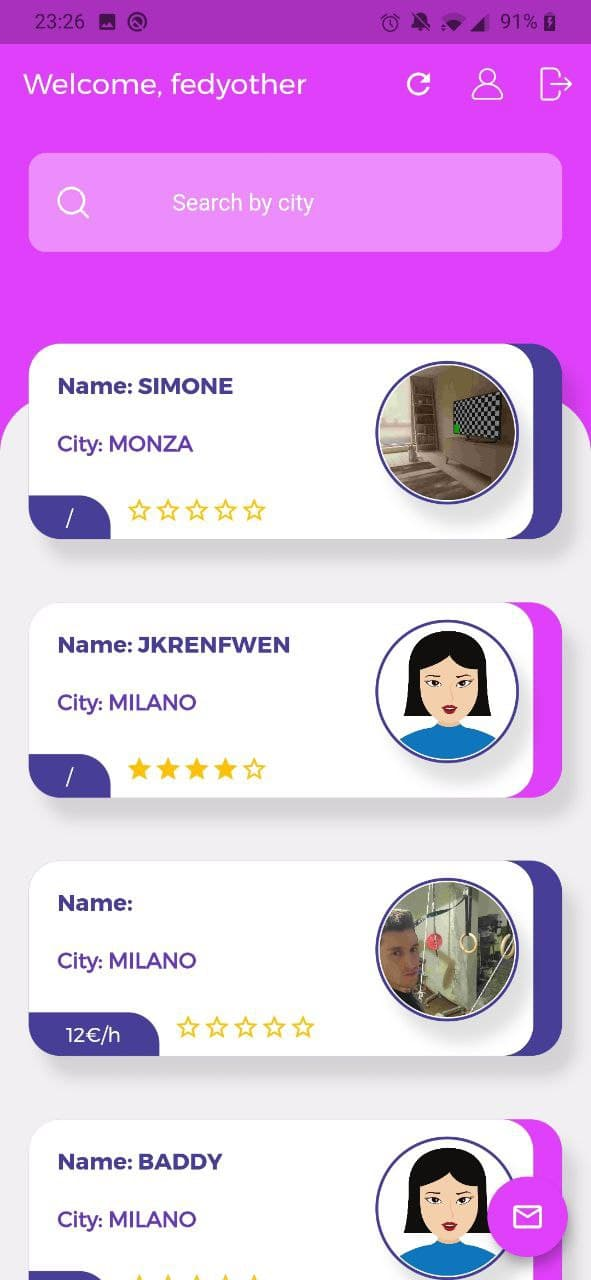
\includegraphics[height=.6\textheight]{../../assets/screens/homepage.jpg}
        \caption{\textbf{Homepage}}\label{fig:figure}
    \end{figure}
    \begin{center}
        The \textbf{Homepage} appears only if the user is correctly authenticated.
        Here a list of available caregivers is shown with all the relevant information.
        You can also search for a specific city.
    \end{center}

    \begin{figure}[H]
        \centering
        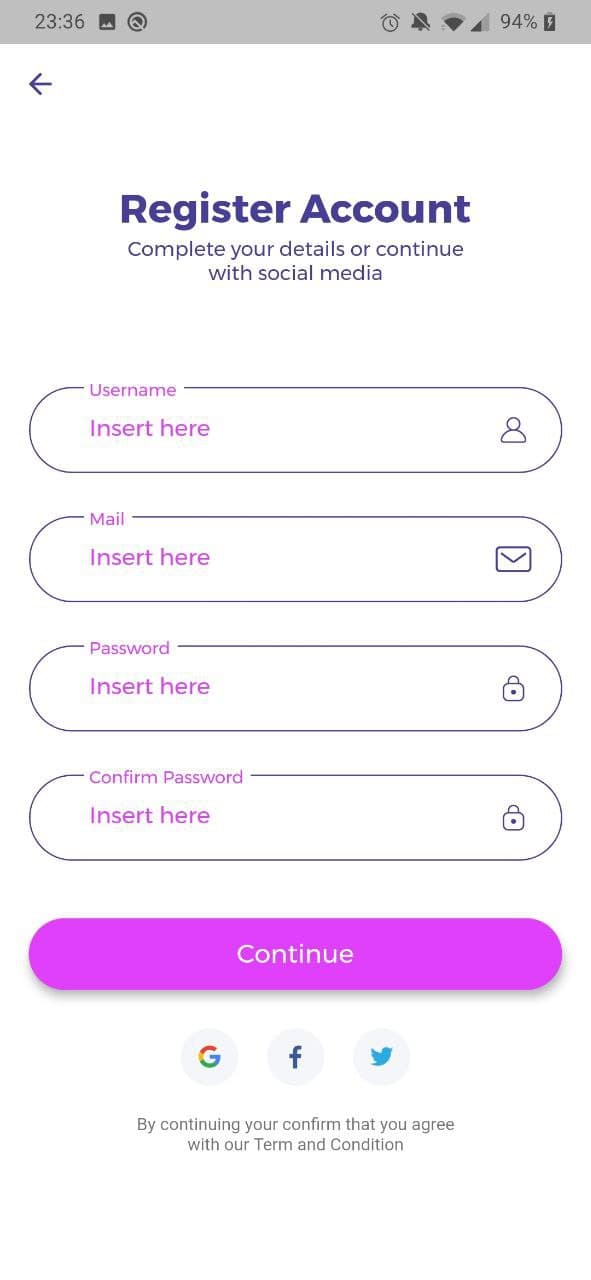
\includegraphics[height=.6\textheight]{../../assets/screens/register.jpg}
        \caption{\textbf{Update Profile Screen}}\label{fig:figure}
    \end{figure}
    \begin{center}
        The \textbf{Update Profile Screen} is accessible only by caregivers, using the top right icon.
        Here the caregiver can update all the information he wants to be visible from others.
    \end{center}

    \begin{figure}[H]
        \centering
        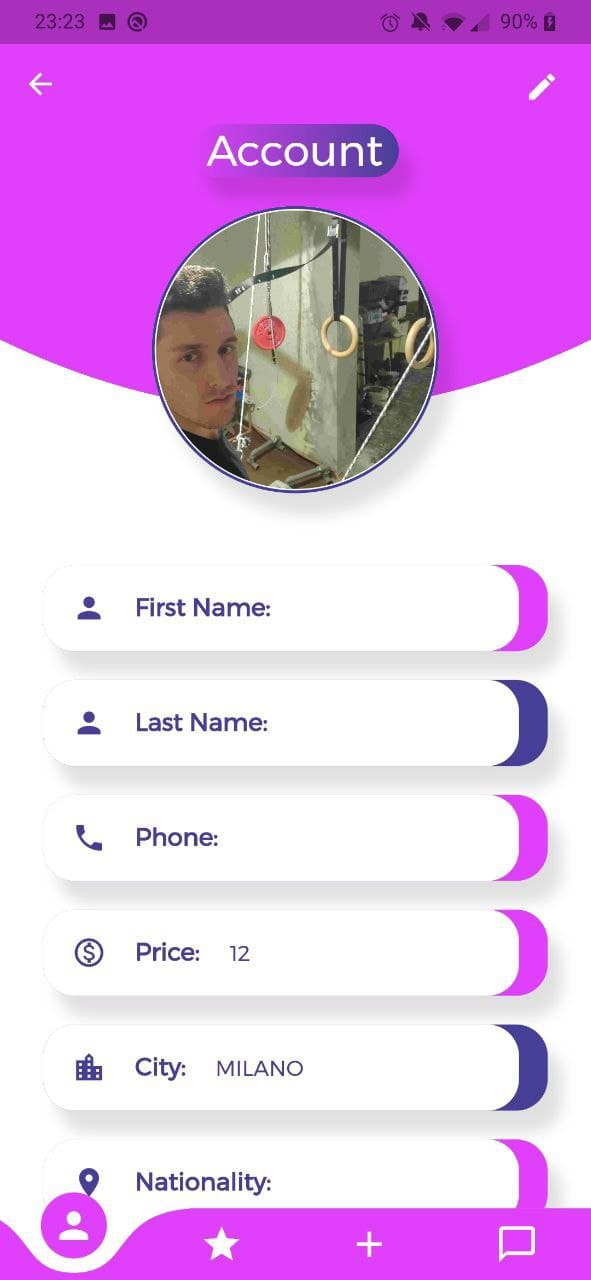
\includegraphics[height=.6\textheight]{../../assets/screens/profile.jpg}
        \caption{\textbf{Profile Screen}}\label{fig:figure}
    \end{figure}
    \begin{center}
        The \textbf{Profile Screen} shows all the information of the selected user from the homepage.
    \end{center}

    \begin{figure}[H]
        \centering
        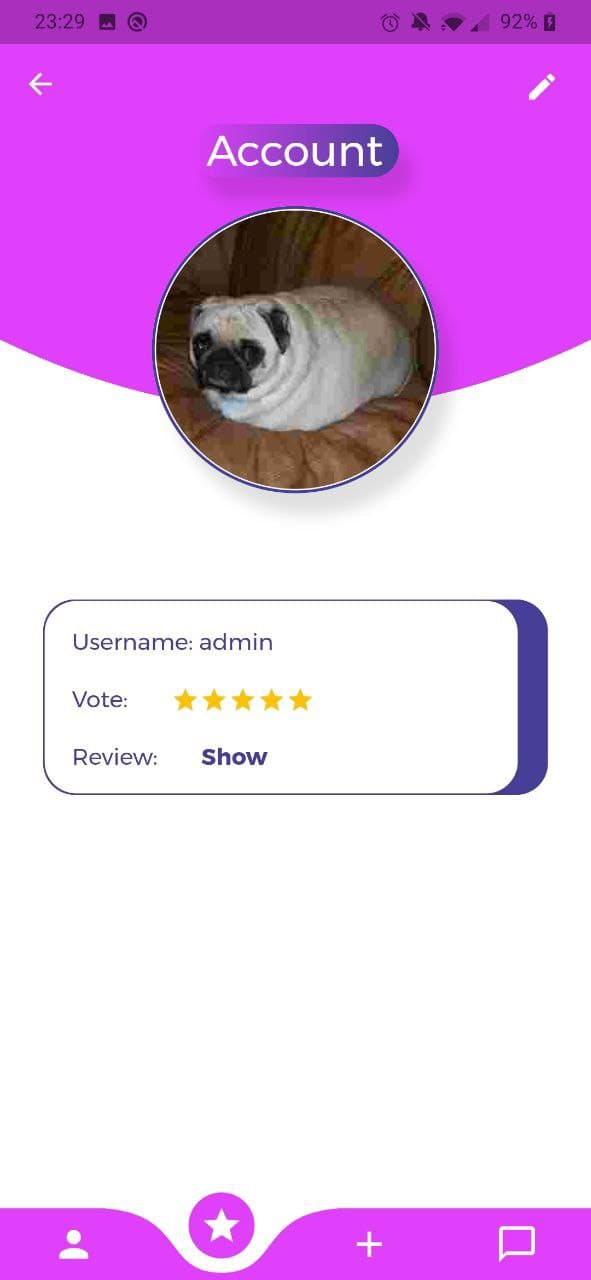
\includegraphics[height=.6\textheight]{../../assets/screens/reviews.jpg}
        \caption{\textbf{Reviews Screen}}\label{fig:figure}
    \end{figure}
    \begin{center}
        The \textbf{Reviews Screen} shows all the reviews a user got from other users.
    \end{center}

    \begin{figure}[H]
        \centering
        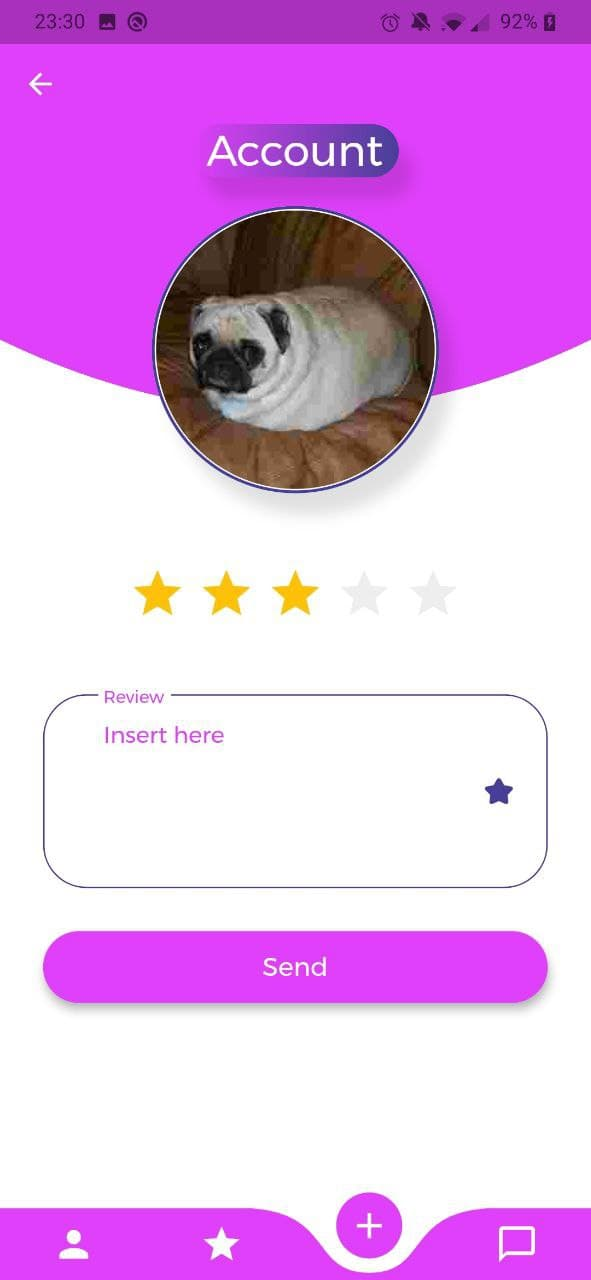
\includegraphics[height=.6\textheight]{../../assets/screens/write_review.jpg}
        \caption{\textbf{Write Review Screen}}\label{fig:figure}
    \end{figure}
    \begin{center}
        The \textbf{Write Review Screen} allows only the standard user to write a review
        and give stars to the selected caregiver.
    \end{center}

\end{document}
